\subsection{Stochastic process}

When describing how a quantity evolves over time with a non-deterministic
trajectory we often use what is commonly known as stochastic processes. For
example imagine we are keeping track of a random variable $X$ that changes over
time. This stochastic variable $X$ could describe things such as count of a
specific chemical species, average price of an asset over a period of time,
frequency of a particular allele on a population, etc. To describe how this
variable $X$ changes over time we could in principle list an infinite number of
functions
\begin{equation}
  X(t) = f(X, t).
\end{equation}
This is what we call a stochastic process, i.e. the time evolution of a random
variable $X$. What we are doing here is considered notation abuse by the more
scrupulous mathematicians. Usually people prefer to define a random process as
$Y_X(t) \equiv f(X, t)$ to specify that we are studying how a random variable
$X$ evolves over time $t$ without compromising the use of $X$ as the sole
random variable, but I personally find that notation too strict. Most of our
efforts in these notes will go into describing the probability distribution of
such processes $P(x, t)$, i.e. the probability of our particular random process
taking the specific value $X(t) = x(t)$. More on that later.

Let's clarify all these subtle but important notation differences: The random
variable $X$ is a mapping from a random event to the real line; in other words,
for a particular quantity that we want to describe we assign a number to
represent the event that happened. A useful example is to think about it as
getting to observe a specific face once we roll a die, and assigning a number
from 1 to 6 to represent the face we observed. The stochastic process $X(t)$
describes the values that our random variable $X$ can take over time. Following
up with the die example this could be rolling a die every so often and keeping
track of the numbers that we obtain. This process $X(t)$ represents the
\textbf{ensemble} of possible realizations $x(t)$. In other words, as shown
schematically in \fref{fig01_00001} $X(t)$ describes all possible values that
the quantity $X$ can take over time, and $x(t)$ describes a specific trajectory
that happened to occur for a specific realization of the process.

\begin{figure}[h!]
	\centering 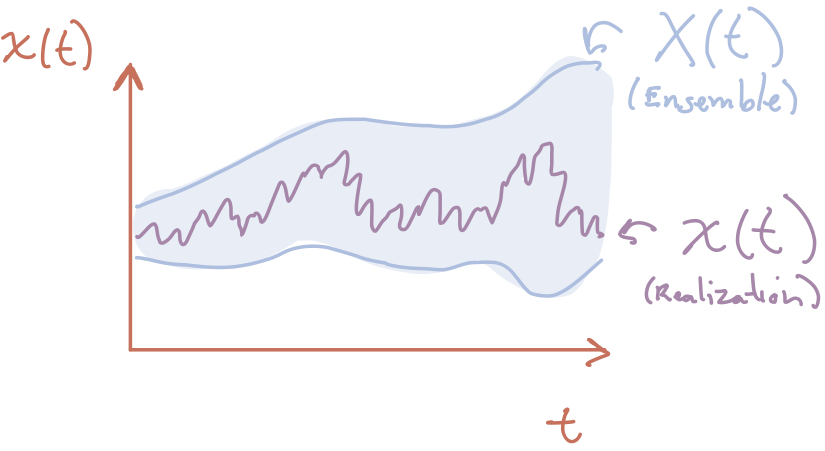
\includegraphics[width=0.5\textwidth]
  {../fig/drift_langevin/01_00001.jpeg}
	\caption{\textbf{Schematic description of a stochastic process}. The shaded
	region describes the stochastic process $X(t)$, i.e. all the possible values
	that the random variable $X$ can take over time. The particular realization
	$x(t)$ describes a specific trajectory that the random variable $X$ took in
	one particular case.}
  \label{fig01_00001}
\end{figure}

From the intuition presented in \fref{fig01_00001} we understand that all
possible trajectories that our stochastic process can take are contained in the
function $X(t)$. But some particular paths $x(t)$ are more likely to happen
than others. This is what the language of probability theory allows us to
compute! In principle we are interested in writing how likely it is for our
process to take a specific value $x(t)$. This is described by the probability
function $P(x, t)$ which will be at the center of our endeavors for these
notes. Once we define our stochastic process we might want to compute a moment
of the distribution. Recall that for a continuous random variable $X$ with
probability density function $P_X(x)$, a moment is defined as
\begin{equation}
  \ee{X^m} \equiv \int dx \; x^m P_X(x),
\end{equation}
where the integral is taken over all the values that $X$ can take. Notice that
our notation for the distribution $P_X(x)$ highlights that we are only
considering values that $X$ can take, no time involved so far. For our case
in which the random variable can change over time what we have to do is settle
for a specific time point $t^*$ and compute the average at that time point
\begin{equation}
  \ee{X(t^*)^m} \equiv \int dx \; x^m P(x, t^*).
  \label{eq_process_moment}
\end{equation}
Notice that this is still not making a statement about the time evolution of
our variable $X$, but rather committing to a specific time point $t^*$ and then
computing the $m\tth$ moment at that time point. An intuitive way to think
about this is to take a frequentist approach for probability. We imagine that
we get to observe many many individual trajectories $\{x_1(t), \ldots
x_n(t)\}$, as schematically shown in \fref{fig01_00002} then what
\eref{eq_process_moment} is doing is computing the moment at a specific time
point $t^*$ highlighted also in \fref{fig01_00002}.

\begin{figure}[h!]
	\centering 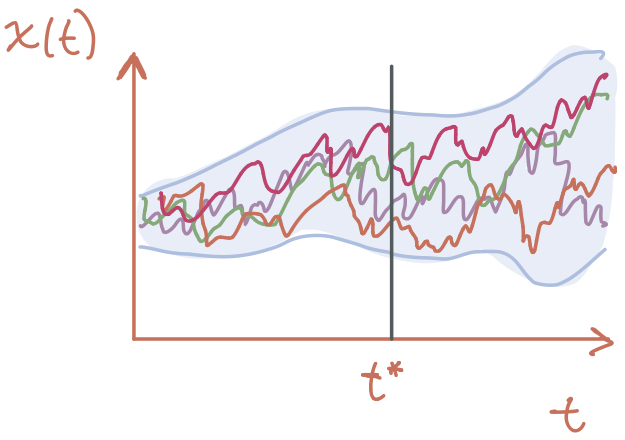
\includegraphics[width=0.5\textwidth]
  {../fig/drift_langevin/01_00002.jpeg}
	\caption{\textbf{Computing a moment of a distribution $\ee{X(t)}$}. Multiple
  realizations of the stochastic process $\{x_1(t), \ldots x_n(t)\}$ are
  highlighted. In the limit where we have many many of these trajectories we
  can then compute a moment of the distribution $P(x, t^*)$ for a specific time
  point $t^*$. \mrm{need better caption}}
  \label{fig01_00002}
\end{figure}

There is no reason why we have to limit ourselves to a single time point $t^*$.
In particular there are interesting quantities such as the autocorrelation
function $\kappa(t_1, t_2)$ that analyze how two different time points $t_1$
and $t_2$ covary with each other. This quantity is defined as
\begin{equation}
  \kappa(t_1, t_2) = \ee{\left(X(t_1) - \ee{X(t_1)}\right)
                         \left(X(t_2) - \ee{X(t_2)}\right)}.
\end{equation}
\mrm{Not sure if I will need to include this if we don't ge to compute moments
that refer to multiple time points.}

Having understood conceptually what stochastic process are and what they allow
us to do we are ready to see their practical implementation. The stochastic
process literature is rich and very formal, but it can be daunting to grasp the
basics of it. For our purposes we will take a more pragmatic approach rather
than diving into the intricacies of the formalism. Our fundamental equation to
model stochastic processes will be the Langevin equation.

\subsection{The Langevin equation}

Since Robert Brown systematically described the jiggling of particles of
organic and inorganic origin under the microscope, physicists of the caliber of
Einstein and Smoluchowski tried to describe the phenomena. The first success
came from Einstein himself who in 1905 published a microscopic description of
Brownian motion at the time where the atomic structure of matter was still up
in the air. In 1908 only three years later, motivated by this theoretical
predictions, Jean Baptiste Perrin experimentally confirmed Einstein's theory to
unambiguously settle the controversy behind the existence of atoms. That same
year Paul Langevin published a seminal paper in which he proposed an
``infinitely simpler'' formulation of Brownian dynamics according to himself.
In doing so Langevin made use of what we know nowadays as a stochastic
differential equation. Ever since, the study of microscopic particles jiggling
under thermal forces has had enormous consequences in our understanding of the
structure of matter, and has motivated the development of the mathematical
formalism of stochastic calculus with great impact in physics, economics, and
as we are concerned here biological evolution.

The mathematical object that Langevin proposed that now carries his name is
different form the standard ordinary differential equations in the sense that
it includes a stochastic term. More specifically for a 1D system the Langevin
equation that describes the dynamics of $x(t)$ is of the form
\begin{equation}
  \dt{x} = A(x, t) + B(x, t) \xi(t),
  \label{eq_langevin}
\end{equation}
where $A(x, t)$ is the directional deterministic field that could depend on the
variable $x$ itself as well as time, $B(x, t)$ is the scale associated with the
stochasticity of the process and $\xi(t)$ is the random variable associated
with the dynamics of $x(t)$. Without the second term on the right-hand side we
have a regular differential equation for which there is most likely a method to
solve it given that $A(x, t)$ is a well behaved function. The solution of 
\eref{eq_langevin} without this second term would be of the form
\begin{equation}
  x(t) = x_o + \int_{t_o}^t dt\; A(x, t),
\end{equation}
where $x_o$ is the initial condition, i.e. $x(t = t_o) = x_o$. This solution
would be a smooth deterministic trajectory for $x(t)$. The extra element that
makes \eref{eq_langevin} special is the stochastic term $B(x, t) \xi(t)$. 
$B(x, t)$ is simply a coefficient that determines the amplitude of the noise,
i.e. it sets the scale for how noisy the stochastic process $x(t)$ must be. But
the true innovative feature of \eref{eq_langevin} is $\xi(t)$, sometimes called
white noise. This term is itself a random variable, meaning that it is defined
by a probability distribution $P(\xi, t)$. The reason this term is called white
noise is because the noise is assumed to have mean zero, i.e. fluctuations that
randomly increase the value of $x(t)$ cancel with fluctuations that tend to
decrease $x(t)$ on average. This is mathematically expressed as
\begin{equation}
  \ee{\xi(t)} = 0.
\end{equation}
The second reason this term is called white noise is because the noise at time
$t$ is independent of the noise at any other point in time $t'$. This is
sometimes referred as delta-correlated noise because the way we express this
lack of time correlation between time points is through a $\delta$-function as
\begin{equation}
  \ee{\xi(t) \xi(t')} = 2D \delta(t - t'),
  \label{eq_noise_delta}
\end{equation}
where the prefactor $2D$ is put to resemble the origins of this equation where
$D$ represented the diffusion coefficient of the Brownian particle. What 
\eref{eq_noise_delta} is saying is that only when $t = t'$ the noise
autocorrelation function takes the magnitude $2D$ - that's what the 
$\delta$-function role is. In other words, independently of what the noise
magnitude was at time $t'$, the noise at time $t$ is sampled from a
distribution with mean $\ee{\xi(t)} = 0$ and variance $\ee{\xi(t)^2} = 2D$.

Since we are characterizing the noise via only its first two moments, i.e. the
noise and the variance, we take the distribution of $\xi(t)$ to be Gaussian.
This assumption is justified because of the central limit theorem that tells us
that the distribution of the sum of many independent random variables tends to
a Gaussian distribution. That means the the probability density function of
$\xi(t)$ is of the form
\begin{equation}
  P(\xi(t)) = {1 \over \sqrt{4 \pi D}} 
  \E^{- {\xi(t)^2 \over 4D}}.
\end{equation}
To get a better feeling for how this equation works let's work through a very
simple example.

\subsubsection{Biased random walk}

In order to see what we can do with this type of mathematical object let's
define the a very simple Langevin equation that includes both a directional
term and the stochastic term. For this we will imagine a small particle
performing a random walk in 1D. We will follow the particle's position $x(t)$
as it is subject to a restoration force and a constant noise term. What this
means is that the dynamics of $x(t)$ are given by
\begin{equation}
  \dt{x} = -\gamma x(t) + \xi(t),
  \label{eq_random_walk_langevin}
\end{equation}
where we set $A(x, t) = -\gamma x(t)$ and $B(x, t) = 1$. If $\xi(t)$ was a
regular function \eref{eq_random_walk_langevin} would be a non-homogeneous
linear differential equation. To solve this equation we could use for example
the integrating factor method. For this we would rewrite
\eref{eq_random_walk_langevin} as
\begin{equation}
  \dt{x} + \gamma x(t) = \xi(t).
\end{equation}
The integrating factor $M(t) $is then given by
\begin{equation}
  M(t) = \E^{\int \gamma \; dt}.
\end{equation}
The integral in the exponent of the integrating factor is a kind of integral
known as an integral function. The reason being that it gives the primitive
argument itself (in this case $t$) without an integration constant. In other
words, the integral should be thought as
\begin{equation}
  \int \gamma \; dt = \int_0^t \gamma ds,
\end{equation}
where the fundamental theorem of calculus tells us that this gives
\begin{equation}
  \int_0^t \gamma ds = \gamma t,
\end{equation}
regardless of the integration lower limit. Multiplying both sides of the
equation by $M(t)$ then gives
\begin{equation}
  \E^{\gamma t} \left[ \dt{x} + \gamma x(t) \right] =
  \E^{\gamma t} \xi(t).
\end{equation}
The integration factor allows us to rewrite the left-hand side as
\begin{equation}
  \dt{}\left[ x(t) \E^{\gamma t} \right] = 
  \E^{\gamma t} \xi(t).
\end{equation}
We can now integrate both sides of the equation from 0 to $t$ to obtain
\begin{equation}
  \int_0^t ds\; {d \over ds}\left[ x(s) \E^{\gamma s} \right] =
  \int_0^t ds \; \E^{\gamma s} \xi(s).
\end{equation}
For the left-hand side we can use the fundamental theorem of calculus to cancel
the integral with the derivative, obtaining
\begin{equation}
  \left. x(s)\E^{\gamma s} \right\vert_{0}^{t} =
  \int_0^t ds \; \E^{\gamma s} \xi(s).
\end{equation}
Substituting the integration limits and solving for $x(t)$ results in
\begin{equation}
  x(t) = x_o \E^{-\gamma t} + 
  \int_0^t ds \; \E^{-\gamma (t - s)} \xi(s).
  \label{eq_random_walk_sol}
\end{equation}
For the second term on the right-hand side we cannot give a close-form
analytical solution given the probabilistic nature of $\xi(t)$. But what we can
do is describe the statistical properties of the trajectories. For example
let's compute the average position of the random walker $\ee{x(t)}$
\begin{equation}
  \ee{x(t)} = \ee{x_o \E^{-\gamma t} + 
  \int_0^t ds \; \E^{-\gamma (t - s)} \xi(s)}.
\end{equation}
Using the linearity of expected values this gives
\begin{equation}
  \ee{x(t)} = x_o \E^{-\gamma t} +
  \int_0^t ds \; \E^{-\gamma (t - s)} \ee{\xi(s)}.
\end{equation}
Since we defined the mean noise $\ee{\xi(t)} = 0$ this results in
\begin{equation}
  \ee{x(t)} = x_o \E^{-\gamma t}.
\end{equation}
From this result we can see that the memory of the initial position decays
exponentially with a typical time-scale of $\tau = {1 \over \gamma}$.

To compute the second moment $\ee{x(t)^2}$ we need to square 
\eref{eq_random_walk_sol}. This results in
\begin{equation}
  x(t)^2 =
  \left( x_o \E^{-\gamma t} + 
  \int_0^t ds \; \E^{-\gamma (t - s)} \xi(s) \right)^2.
\end{equation}
Expanding the binomial on the right-hand side gives
\begin{equation}
   x(t)^2 = x_o^2 \E^{-2\gamma t} +
   2 x_o \E^{-\gamma t} 
   \left( \int_0^t ds\; \E^{-\gamma (t - s)} \xi(s) \right) +
   \left( \int_0^t ds \; \E^{-\gamma(t - s)} \xi(s) \right)^2.
\end{equation}
We can rewrite the squared integral term as a double integral of the form
\begin{equation}
   \left( \int_0^t ds \; \E^{-\gamma(t - s)} \xi(s) \right)^2 =
   \int_0^t ds \; \int_0^t dz\; \E^{-\gamma (t - s)} \E^{-\gamma (t - z)}
   \xi(s) \xi(z).
\end{equation}
Using this result and taking the expected value results in
\begin{equation}
  \ee{x(t)^2} = \ee{
   x_o^2 \E^{-2\gamma t} +
   2 x_o \E^{-\gamma t} 
   \left( \int_0^t ds\; \E^{-\gamma (t - s)} \xi(s) \right) +
   \int_0^t ds \; \int_0^t dz\; \E^{-\gamma (t - s)} \E^{-\gamma (t - z)}
   \xi(s) \xi(z)
  }.
\end{equation}
We can again use the linearity of expected value. The first term on the
right-hand side involves no random variable $\xi(t)$, so it comes out of the
expected value operator. The second term involves a term $\ee{\xi(s)}$ which we
defined to be zero, so this term will cancel. For the last term we have a term
of the form $\ee{\xi(s)\xi(z)}$ - we defined this to be $2D \delta (s - z)$.
Let's substitute these results
\begin{equation}
  \ee{x(t)^2} = 
   x_o^2 \E^{-2\gamma t} +
   \int_0^t ds\; \int_0^t dz\; \E^{-\gamma (t-s)} \E^{-\gamma (t-z)}
   (2D \delta(s - t)).
\end{equation}
Now that we have this $\delta$-function in place we can evaluate the integral
over the values of $z$. The $\delta$-function means that only when $z = s$ this
term contributes; in practice this means that the result from the integral over
$z$ is to substitute all values of $z$ for $s$. This looks like
\begin{equation}
  \ee{x(t)^2} = 
   x_o^2 \E^{-2\gamma t} +
   2D \int_0^t ds \; \E^{-\gamma (t-s)} \E^{-\gamma (t-s)}.
\end{equation}
Factorizing the terms with exponent $t$ and taking them out of the integral
results in
\begin{equation}
   \ee{x(t)^2} = 
   x_o^2 \E^{-2\gamma t} +
   2D \E^{-2 \gamma t} \int_0^t ds\; \E^{2 \gamma s}.
\end{equation}
Evaluating the integral results in
\begin{equation}
   \ee{x(t)^2} = 
   x_o^2 \E^{-2\gamma t} +
   {2D \E^{-2\gamma t} \over 2 \gamma}\left( \E^{2 \gamma t} - 1 \right).
\end{equation}
This can be simplified to
\begin{equation}
   \ee{x(t)^2} = 
   x_o^2 \E^{-2\gamma t} +
   {D \over \gamma} \left( 1 - \E^{-2 \gamma t} \right).
\end{equation}

Now that we have the first and the second moment we can compute the variance of
our random walk. Recall that the variance is given by
\begin{equation}
  \sigma^2(x(t)) = \ee{x(t)^2} - \ee{x(t)}^2.
\end{equation}
Using the results we derived results in
\begin{equation}
  \sigma^2(x(t)) = x_o^2 \E^{-2\gamma t} +
   {D \over \gamma} \left( 1 - \E^{-2 \gamma t} \right) -
   x_o^2 \E^{-2\gamma t} = 
   {D \over \gamma} \left( 1 - \E^{-2 \gamma t} \right).
\end{equation}
In the limit where $t \rightarrow \infty$ we the find that the variance
converges to $\sigma^2(x) = {D \over \gamma}$.